\documentclass[11pt]{standalone}

\usepackage{helvet}

\usepackage{ifthen}
\usepackage{tikz} 
\usetikzlibrary{shapes.misc}
\usetikzlibrary{arrows,arrows.meta}
\usetikzlibrary{calc,intersections, patterns, math}

\definecolor{pfeil}{RGB}{168,167,167}
\definecolor{petrol}{RGB}{0, 118, 136}
\definecolor{darkgoldenrod}{RGB}{184, 134, 11}
\colorlet{petrol-lighter}{petrol!40}
\colorlet{darkgoldenrod-lighter}{darkgoldenrod!40}

\begin{document}

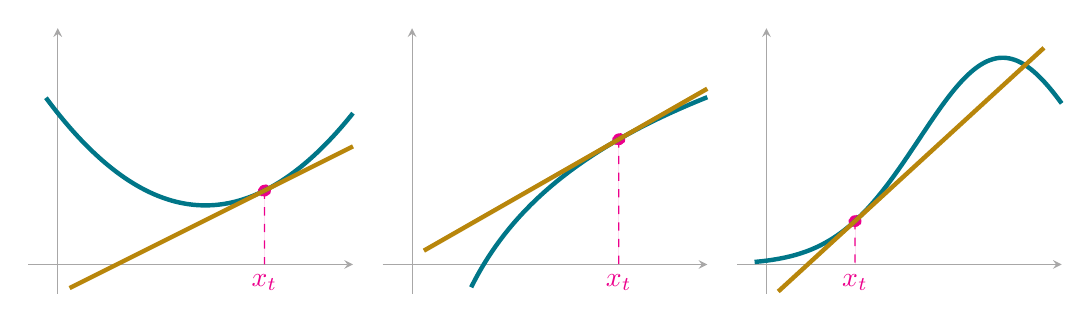
\begin{tikzpicture}[pfeil, scale=1.5]

    % \draw[thick, fill=petrol!20, draw=petrol-lighter, rounded corners=2ex, opacity=0.5] (0,0) rectangle ++ (1.5,3.5);
    % \draw[thick, fill=darkgoldenrod!20, draw=darkgoldenrod-lighter, rounded corners=2ex, opacity=0.5] (5,0) rectangle ++ (1.5,3.5);

    \draw[-stealth] (-0.25,0) -- (2.5,0);
    \draw[-stealth] (0,-0.25) -- (0,2);

    \draw[dashed, magenta, fill] (1.75,0.625) circle (0.05) (1.75,0.625) -- (1.75,0) node[below] {$x_t$};

    \draw[ultra thick,domain=-0.1:2.5, smooth, samples=50, petrol] plot(\x,{0.5*(\x-1.25)^2+0.5});

    \draw[ultra thick,domain=0.1:2.5, smooth, samples=50, darkgoldenrod] plot(\x,{0.5*\x-0.25});
    
    \begin{scope}[shift={(3,0)}]
        \draw[-stealth] (-0.25,0) -- (2.5,0);
        \draw[-stealth] (0,-0.25) -- (0,2);

        \draw[dashed, magenta, fill] (1.75,1.0596) circle (0.05) (1.75,1.0596) -- (1.75,0) node[below] {$x_t$};

    \draw[ultra thick,domain=0.5:2.5, smooth, samples=50, petrol] plot(\x,{ln(\x)+0.5});

    \draw[ultra thick,domain=0.1:2.5, smooth, samples=50, darkgoldenrod] plot(\x,{0.571429*\x+0.0596158});

    \end{scope}
    
    \begin{scope}[shift={(6,0)}]
        \draw[-stealth] (-0.25,0) -- (2.5,0);
        \draw[-stealth] (0,-0.25) -- (0,2);
        
        \draw[dashed, magenta, fill] (0.75,0.3668) circle (0.05) (0.75,0.3668) -- (0.75,0) node[below] {$x_t$};

    \draw[ultra thick,domain=-0.1:2.5, smooth, samples=50, petrol] plot(\x,{1.75*exp(-(\x-2)^2)});

    \draw[ultra thick,domain=0.1:2.35, smooth, samples=50, darkgoldenrod] plot(\x,{0.91705*\x-0.320967});
    \end{scope}
    

\end{tikzpicture}

\end{document}
